Verwenden Sie das Pumping Lemma um zu zeigen, dass die Sprache
\[
L
=
\{
\texttt{0}^n\texttt{1}^m
\mid
0<n<m
\}
\]
nicht regulär ist.
Was ändert sich an Ihrem Beweis, wenn nicht nur $n<m$ gefordert wird,
sondern $n+1<m$.

\begin{loesung}
\definecolor{darkgreen}{rgb}{0,0.6,0}
\begin{enumerate}
\item
Wir nehmen an, $L$ sei regulär.
\item
Nach dem Pumping Lemma gibt es eine Zahl $N$ derart, dass Wörter
mit Länge $\ge N$ aufpumpbar sind.
\item
Wir verwenden das Wort $\texttt{0}^N\texttt{1}^{N+1}\in L$
\item
Gemäss Pumping Lemma muss es aufteilbar sein in $w=xyz$, wobei $|xy|\le N$
und $|y|>0$.
\begin{center}
\def\s{0.6}
\def\punkt#1#2{({(#1)*\s},{(#2)*\s})}
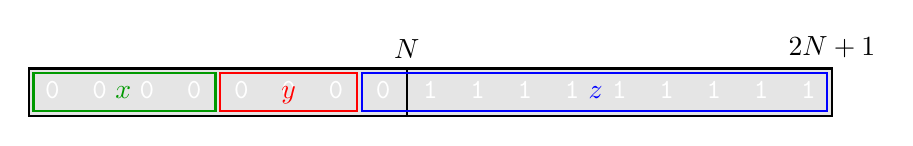
\begin{tikzpicture}[>=latex,thick]
\fill[color=gray!20] \punkt{0}{0} rectangle \punkt{17}{1};
\draw \punkt{0}{0} rectangle \punkt{17}{1};
\draw \punkt{8}{0} -- \punkt{8}{1};
\foreach \x in {0.5,1.5,...,7.5}{
	\node[color=white] at \punkt{\x}{0.5} {\texttt{0}\strut};
}
\foreach \x in {8.5,9.5,...,16.5}{
	\node[color=white] at \punkt{\x}{0.5} {\texttt{1}\strut};
}
\node at \punkt{8}{1} [above] {$N$};
\node at \punkt{17}{1} [above] {$2N+1$};
\draw[color=darkgreen] \punkt{0.1}{0.1} rectangle \punkt{3.95}{0.9};
\node[color=darkgreen] at \punkt{2}{0.5} {$x\mathstrut$};
\draw[color=red] \punkt{4.05}{0.1} rectangle \punkt{6.95}{0.9};
\node[color=red] at \punkt{5.5}{0.5} {$y\mathstrut$};
\draw[color=blue] \punkt{7.05}{0.1} rectangle \punkt{16.9}{0.9};
\node[color=blue] at \punkt{12}{0.5} {$z\mathstrut$};
\end{tikzpicture}
\end{center}
\item Der Teil $\color{red}y$  kann aufgepumpt werden, wobei sich 
das folgende Wort ergibt
\begin{center}
\def\s{0.6}
\def\punkt#1#2{({(#1)*\s},{(#2)*\s})}
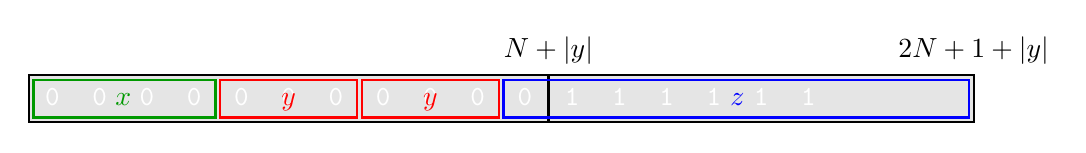
\begin{tikzpicture}[>=latex,thick]
\fill[color=gray!20] \punkt{0}{0} rectangle \punkt{20}{1};
\draw \punkt{0}{0} rectangle \punkt{20}{1};
\draw \punkt{11}{0} -- \punkt{11}{1};
\foreach \x in {0.5,1.5,...,10.5}{
	\node[color=white] at \punkt{\x}{0.5} {\texttt{0}\strut};
}
\foreach \x in {11.5,12.5,...,16.5}{
	\node[color=white] at \punkt{\x}{0.5} {\texttt{1}\strut};
}
\node at \punkt{11}{1} [above] {$N+|y|$};
\node at \punkt{20}{1} [above] {$2N+1+|y|$};
\draw[color=darkgreen] \punkt{0.1}{0.1} rectangle \punkt{3.95}{0.9};
\node[color=darkgreen] at \punkt{2}{0.5} {$x\mathstrut$};
\draw[color=red] \punkt{4.05}{0.1} rectangle \punkt{6.95}{0.9};
\node[color=red] at \punkt{5.5}{0.5} {$y\mathstrut$};
\draw[color=red] \punkt{7.05}{0.1} rectangle \punkt{9.95}{0.9};
\node[color=red] at \punkt{8.5}{0.5} {$y\mathstrut$};
\draw[color=blue] \punkt{10.05}{0.1} rectangle \punkt{19.9}{0.9};
\node[color=blue] at \punkt{15}{0.5} {$z\mathstrut$};
\end{tikzpicture}
\end{center}
Der \texttt{0}-Teil hat $N+|y|$ Nullen, der \texttt{1}-Teil hat $N+1$
Einsen.
Weil $|y|\ge 1$ ist, $N+|y|\ge N+1$ und nicht mehr $N+|y|<N+1$ wie von
der Sprachdefinition verlangt.
Das aufgepumpte Wort ${\color{darkgreen}x}{\color{red}y}^2{\color{blue}z}$
ist also nicht mehr in der Sprache.
\item
Dieser Widerspruch zeigt, dass die Annahme, $L$ sei regulär, nicht haltbar ist.
\end{enumerate}
Wenn $n+k<m$ gefordert wird, reicht es nicht mehr, nur einmal aufzupumpen,
wenn $|y|=1$ ist.
Aber mit $k$-maligem Aufpumpen wird der gewünschte Effekt immer erreicht.
\end{loesung}
